\chapter{驾驶人行为特性实验}


%\[D = ct/2\]

本文的驾驶人行为特性实验目的在于,调查和记录专业驾驶人与非专业驾驶人在城市路段行车时,采取的跟驰驾驶行为。为分析驾驶人行为特性的异同及其对城市路段交通流的影响提供数据。实验拟获取的数据主要包括实验驾驶人的速度、加速度、以及实验车辆与其前方行驶车辆的相互位置与运动关系。


%\begin{equation}
%D = 2R{\rm{asin}}(\sqrt {\sin _{}^2(\frac{{{l_1} - {l_2}}}{2}) + \cos ({l_1})\cos ({l_2}){{\sin }^2}(\frac{{{w_1} - {w_2}}}{2})} )
%\end{equation}

\section{实验设计}
为了获得实验驾驶人的速度、加速度、以及实验车辆与其前方行驶车辆的相互位置与运动关系,本文使用主动模式的跟驰实验系统进行实际交通环境下的测试。实验系统的软硬件组成描述如下。
%\subsection{实验获取的数据}
%实验获取的数据包括,驾驶人行车过程中,本车与前后车实时保持的距离,即$S_{\text{前}}$、$S_{\text{后}}$;本车的实时速度$V$,前车的实时速度$V_{\text{前}}$;后车的实时速度$V_{\text{后}}$;本车与前车相对速度${\Delta}S_{\text{前}}$;本车与后车相对速度v’后;本车换道频率n,换道时相邻车道提供的前后车距离s换等。
\subsection{硬件组成设备}
如\autoref{equipment},实验设备包括汽车一辆(手动档)、车载激光测速测距仪一体化系统一套(车载激光测距仪、GPS接收器一个、处理机一台)、摄像机一台、笔记本电脑一台。主要硬件设备如\autoref{allequip}

\begin{figure}[htpb]
\centering
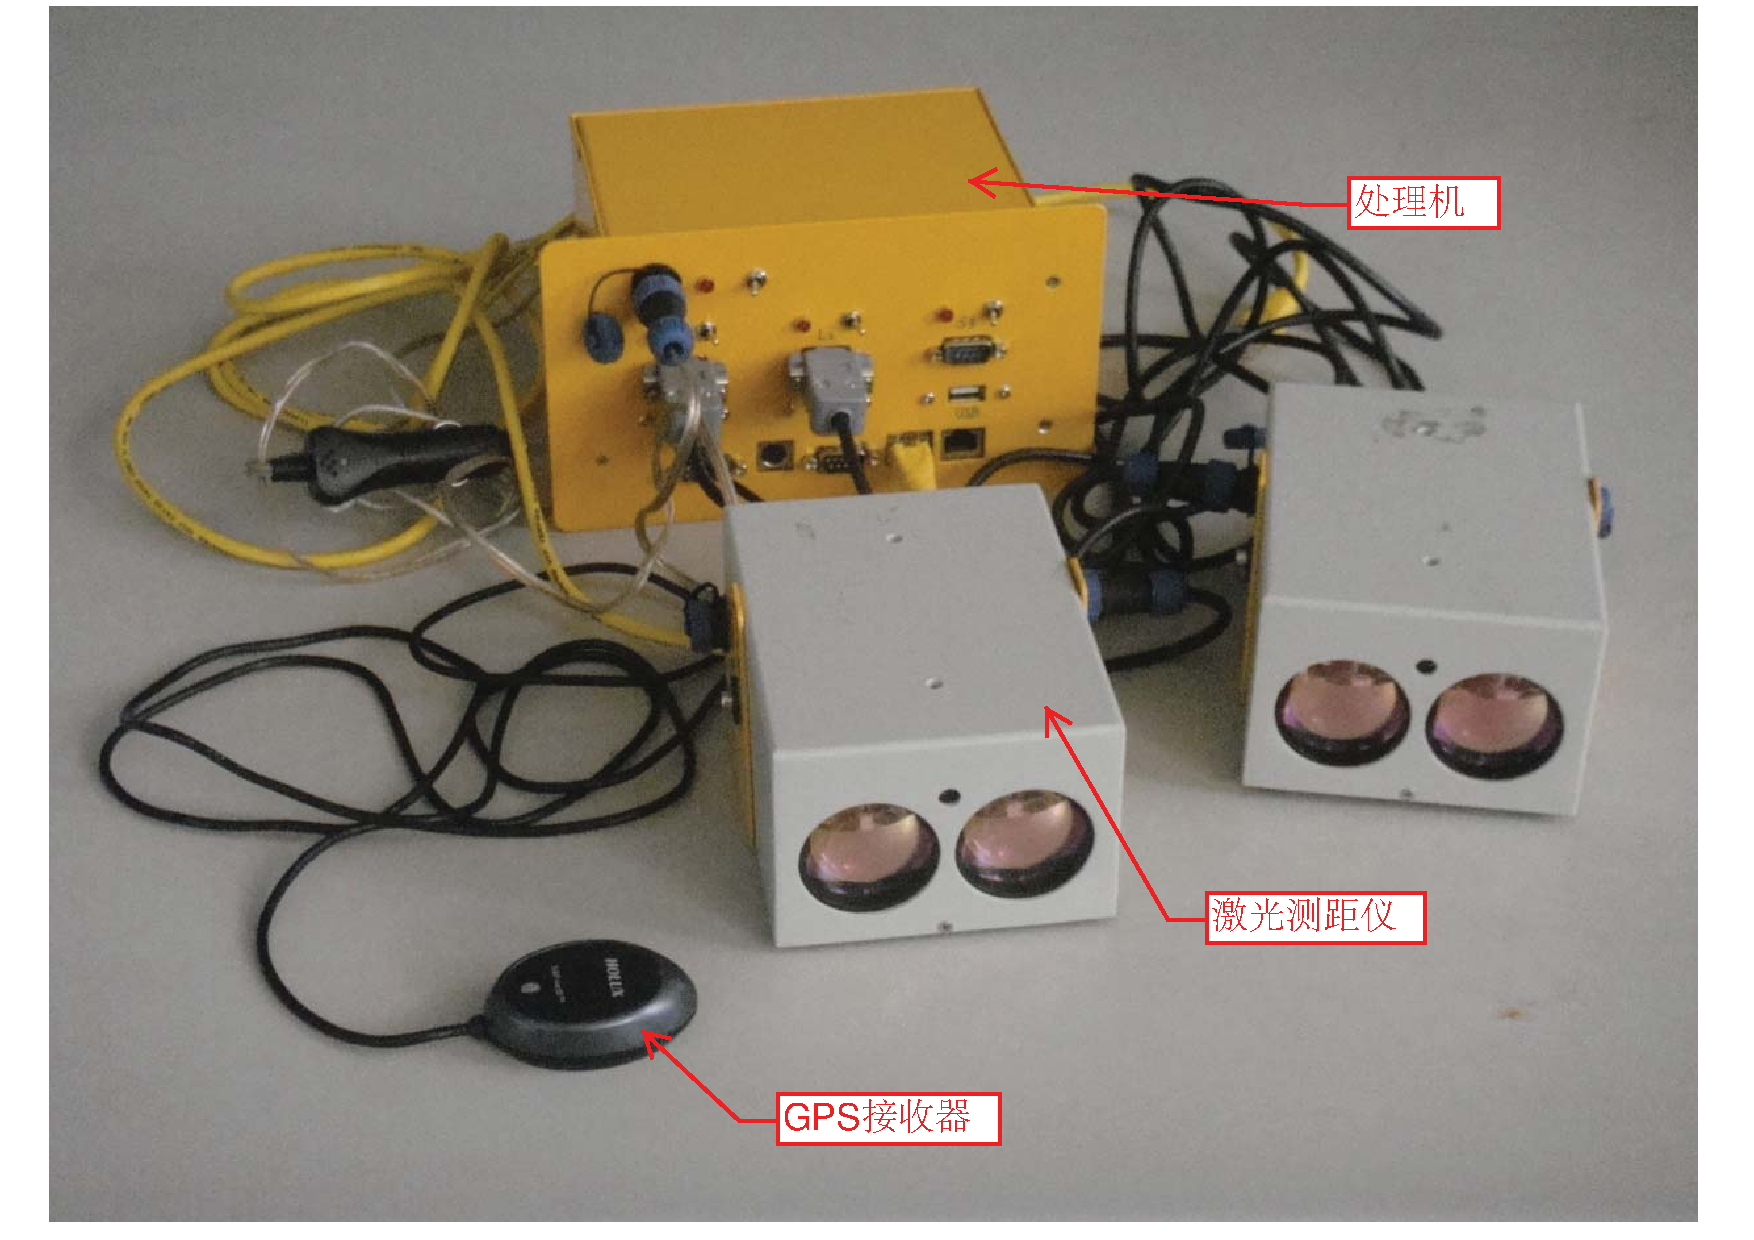
\includegraphics[angle=270,width=0.7\linewidth]{allequip}
\caption{主要硬件设备图}
\label{allequip}
\end{figure}

\begin{table}[htbp]
 \centering
 \caption{硬件设备列表}
 \begin{tabular}{cccc}
   \addlinespace
    \toprule
    序号 & 名称  & 构成 & 用途 \\
    \midrule
	1 & 汽车 & 手动档汽车 & 实验用车 \\
	2 & 车载激光测速测距仪 & 车载激光测距仪、GPS、处理机 & 获取实时车速、车间距 \\
	3 & 摄像机 & 摄像机 & 实验场景记录 \\
	4 & 笔记本电脑 & Thinkpad T40笔记本 & 现场控制终端 \\
    \bottomrule
    \end{tabular}
  \label{equipment}
\end{table}



其中,汽车选取目前道路比较有代表性的车型,北京现代的sonata领翔 2.0 GL MT,其基本参数如\autoref{car_spec}.


\begin{table}[htbp]
  \centering
  \caption{实验车基本参数}
    \begin{tabular}{rr}
    \addlinespace
    \toprule
	指标&	数值\\
	\midrule
    最高车速(Km/h) & 204 \\
    0-100km/n加速时间(s) & 9.9 \\
    车重(kg)    & 1492 \\
    排量(L) & 2.0  \\
    最大马力(ps) & 165 \\
    功率(Kw(ps)/rpm) & 121/6200 \\
    最大扭矩(N·m/rpm) & 197/4600 \\
    \bottomrule
    \end{tabular}%
  \label{car_spec}%
\end{table}%


%\subsection{实验原理}
%通过获取实时连续的本车与前后车的距离以及本车的实时速度,可以推算得到本车与前车和后车的相对速度、前后车的实时速度等相关数据,应用摄像机可以得到本车的换道频率,最后经过数据的处理分析,可以得到换道时本车道前后车的距离,以及换道时相邻车道提供的前后车距离等。
\subsubsection{激光测距基本原理}
激光测距仪是指利用射向目标的激光脉冲或连续波激光束测量目标距离的距离测量仪。它由三大部分组成:激光发射机、激光接收机、电源。激光发射机由脉冲激光器、发射光学系统、取样器以及瞄准光学系统组成,其作用是将高峰值功率的激光脉冲射向目标。激光接收机由接受光学系统、光电探测器和放大器、接收电路组成,其作用是接收从目标漫反射回来的激光脉冲回波并计算和显示目标距离。电源用于设备的供电。
激光测距仪的工作原理是利用脉冲激光器向目标发射单次激光脉冲,计数器测量激光脉冲到达目标并由目标 返回到接收机的往返时间,由此运算目标的距离。计算公式为:

\begin{equation}
D = ct/2
\end{equation}

其中$D$是与目标的距离, $c$为光速,$t$是光往返时间。

激光测距仪的工作过程是:首先瞄准目标,然后接通激光电源,起动激光器,通过发射光学系统,向瞄准的目标发射激光脉冲信号。同时,采样器采集发射信号,作为计数器开门的脉冲信号,起动计数器,钟频振荡器向计数器有效的输入钟频脉冲,由目标反射回来的激光回波经过大气传输,进入接收光学系统,作用在光电探测器上,转变为电脉冲信号,经过放大器放大,进入计数器,作为计算器的关门信号,计数器停止技术。计数器从开门到关门期间,所进入的钟频脉冲个数,经过运算得到目标距离。


\subsubsection{GPS卫星定位系统基本原理}
GPS系统由空间部分、地面监控部分和用户端三个部分组成。

(1)GPS的空间部分:由21颗工作卫星和3颗备用卫星组成,24颗卫星均匀覆盖在地球上空,可以保证地球上所有地点任意时刻都能同时看到至少4颗GPS卫星。

(2)GPS的地面监控部分:地面监控设备的作用是监测和控制卫星上的各种设备是否正常工作,以及卫星是否一直沿着预定轨道运行;另一作用是保持各颗卫星处于同一时间标准——GPS时间系统。GPS地面监控系统包括一个主控站、三个注入站和五个监测站。

(3)GPS的用户端:即是GPS的信号接收机,它能捕获卫星的信号,对所接收的GPS信号进行变换、放大和处理,实时地计算出测点的三维位置、速度和时间。

GPS系统的基本原理是:太空中的卫星在任意时刻都有一个坐标值(星历为已知值),接收机所在位置为未知值,信息在传送过程中,所需耗费的时间,可经由比对卫星时钟与接收机内的时钟计算之,将此时间差值乘以电波传送速度(一般为光速),就可计算出卫星与接收机间的距离,如此就可依三角向量关系来列出一个相关的方程式,每接收到一颗卫星就可列出一个相关的方程式,因此收到至少三颗卫星信号,即可计算出经纬度坐标,收到四颗则加上高程值,五颗以上更可提高准确度。当接收机处于动态时,每一秒钟的坐标数据都在更新中,也就是说接收机会自动不断地接收卫星信号,并实时地计算其所在位置的坐标数据。系统再将获取的空间与时间的数据结合,计算出车辆的实时速度。

\subsubsection{设备安装}
车载激光测距仪固定在实验车辆挡风玻璃后面,中控台中央的位置,激光头向前放置,能够使激光照射到实验车辆前方的物体,其安装如\autoref{mounted}所示;车载GPS固定在车辆中间的位置;处理机和笔记本电脑放置在车辆后排座位上;摄像机固定在实验车辆后排座位靠背的中间位置上,可以通过实验车辆挡风玻璃拍摄到前方的道路交通情况。


\begin{figure}[htpb]
	\centering
	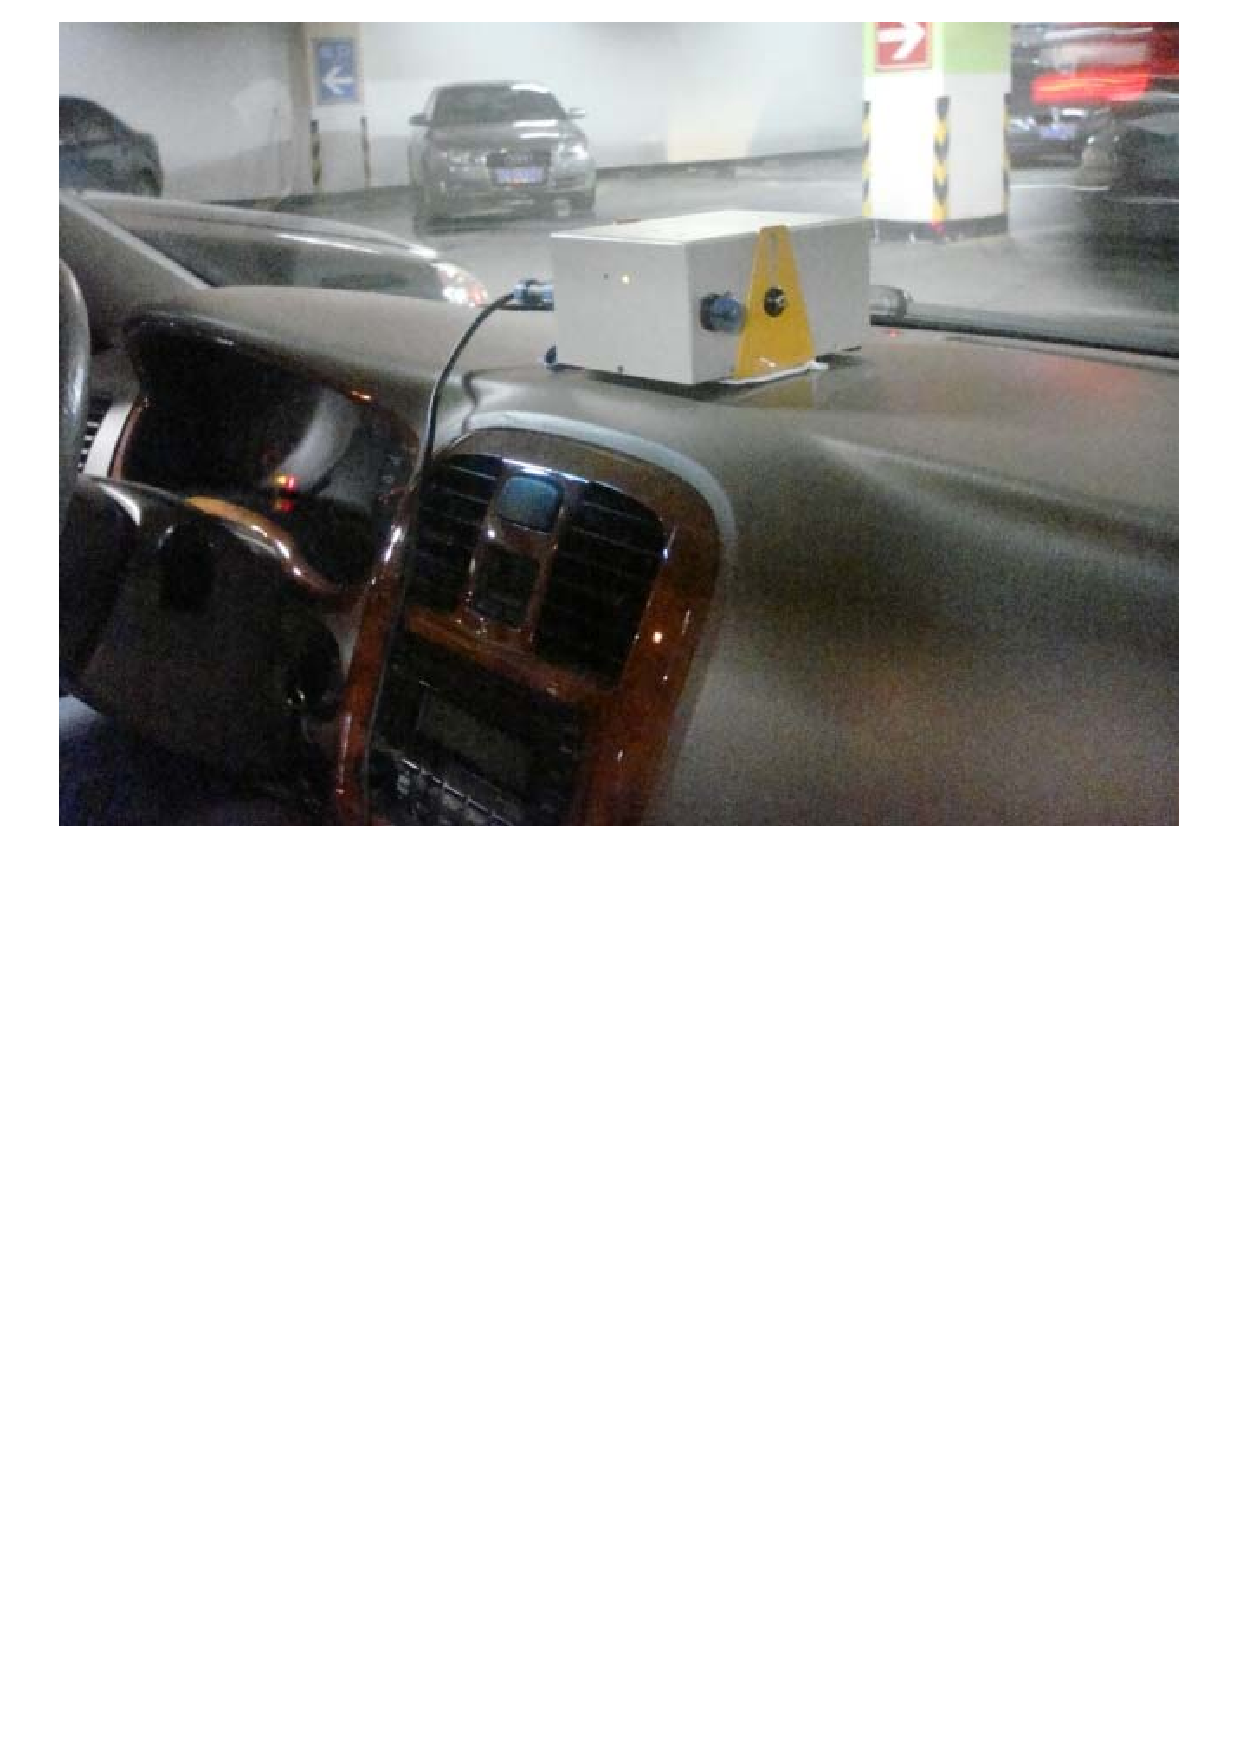
\includegraphics[width=0.7\linewidth]{mounted}
	\caption{设备安装示意图}
	\label{mounted}
\end{figure}



%\subsubsection{车载GPS定位仪系统工作流程}

\subsubsection{车载激光测距测速系统的工作流程}

%激光间距测量仪相比其它测距仪,激光测距仪具有测距精度高、测距速度快、轻小灵活、测量距离数字显示、操作简单等优点。下面分别介绍车载激光的硬件系统和软件系统。

系统包括车载电源、GPS接收器、激光测距系统、处理机及相关配套设施。其中车载电源为激光测距仪和处理机供电,GPS接收器和激光测距仪连接于处理机上,处理机与笔记本电脑相连。数据经过处理机计算传送到笔记本电脑上显示并储存。

驾驶人驾驶实验车在道路上行驶时,车载GPS实时接收卫星信号获取车辆实时的经度与纬度,车载激光测距仪获取与前方物体的距离,车载GPS和车载激光测距仪分别将数据传输至处理机,经过处理机运算处理后将各项数据传输到与处理机相连的笔记本电脑中显示并储存。系统工作流程如\autoref{workflow}所示。

完整的实验系统示意图如\autoref{test_illus}。

\begin{figure}[htpb]
	\centering
	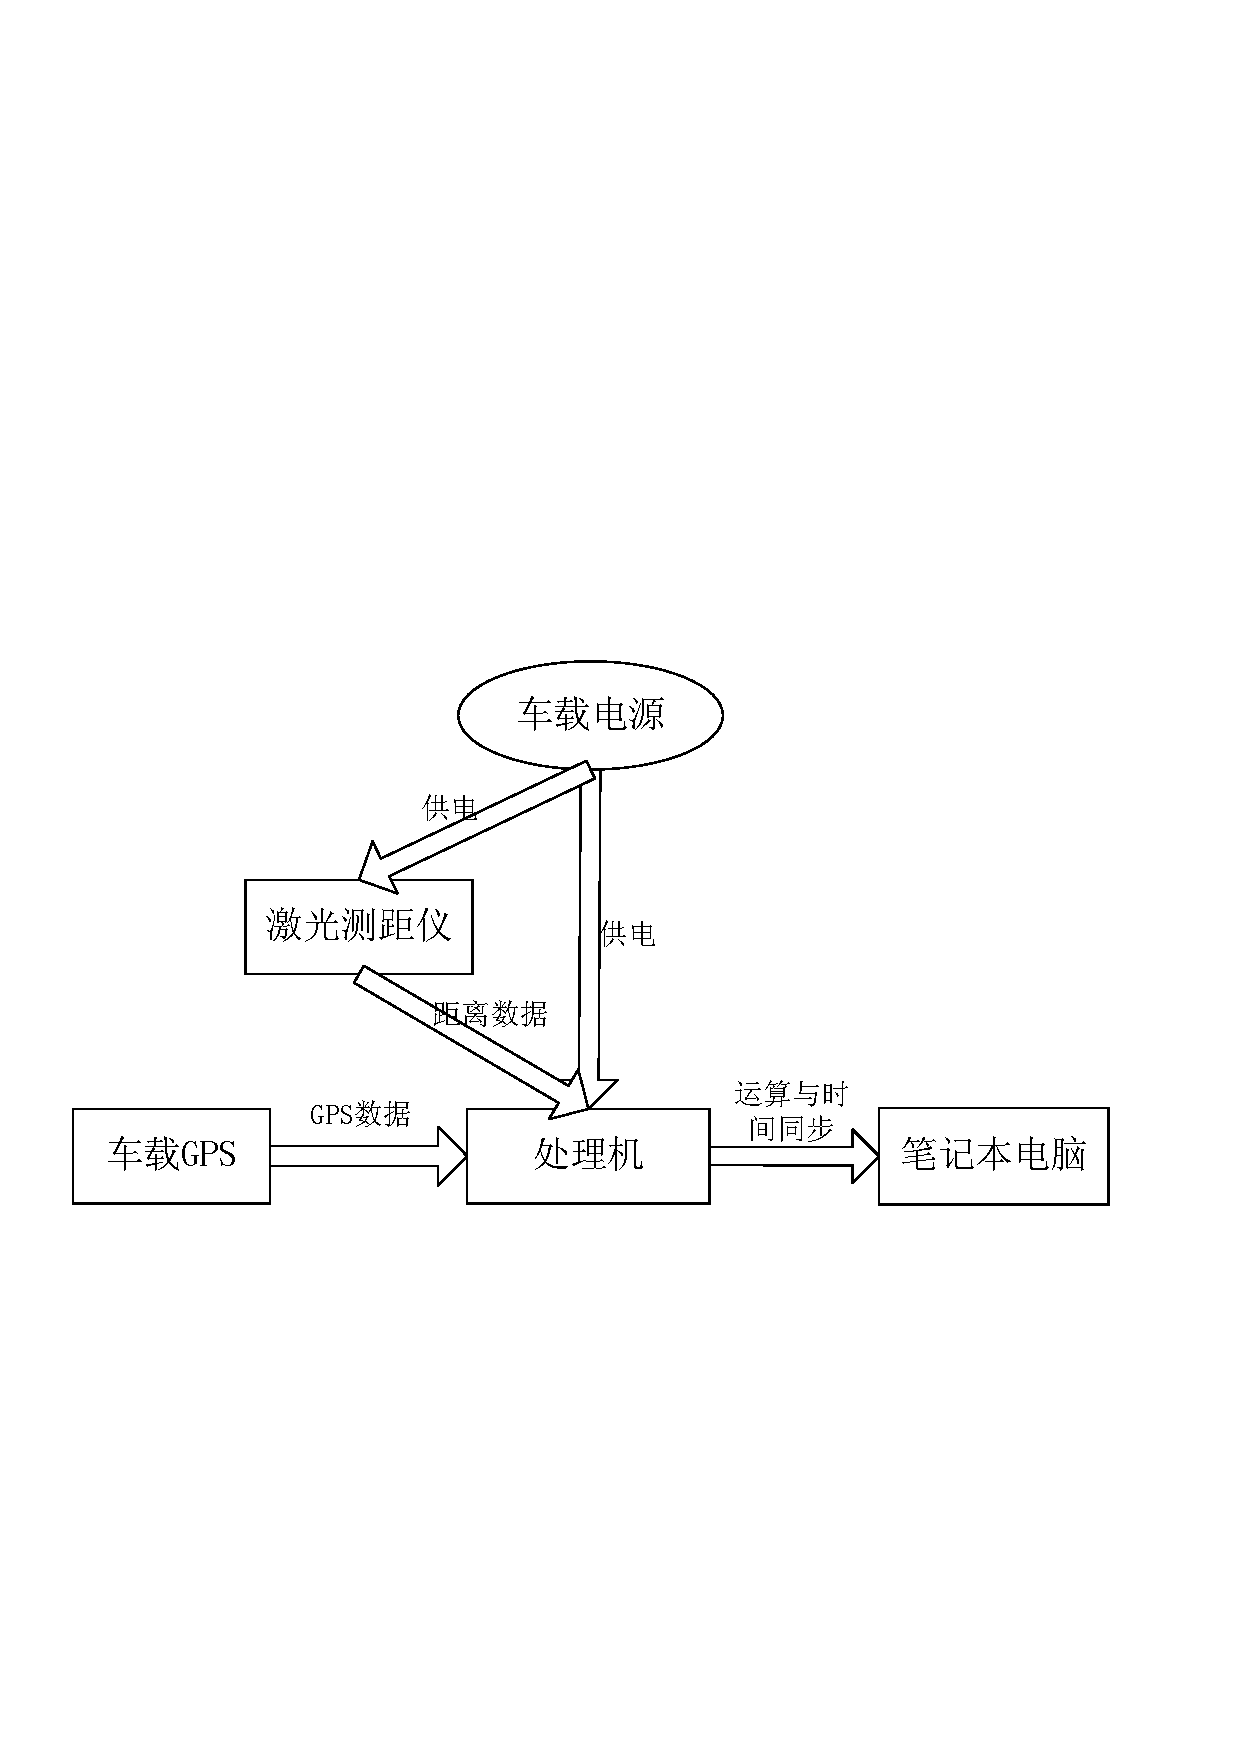
\includegraphics[width=0.7\linewidth]{workflow}
	\caption{系统工作流程示意图}
	\label{workflow}
\end{figure}

\begin{figure}[htpb]
	\centering
	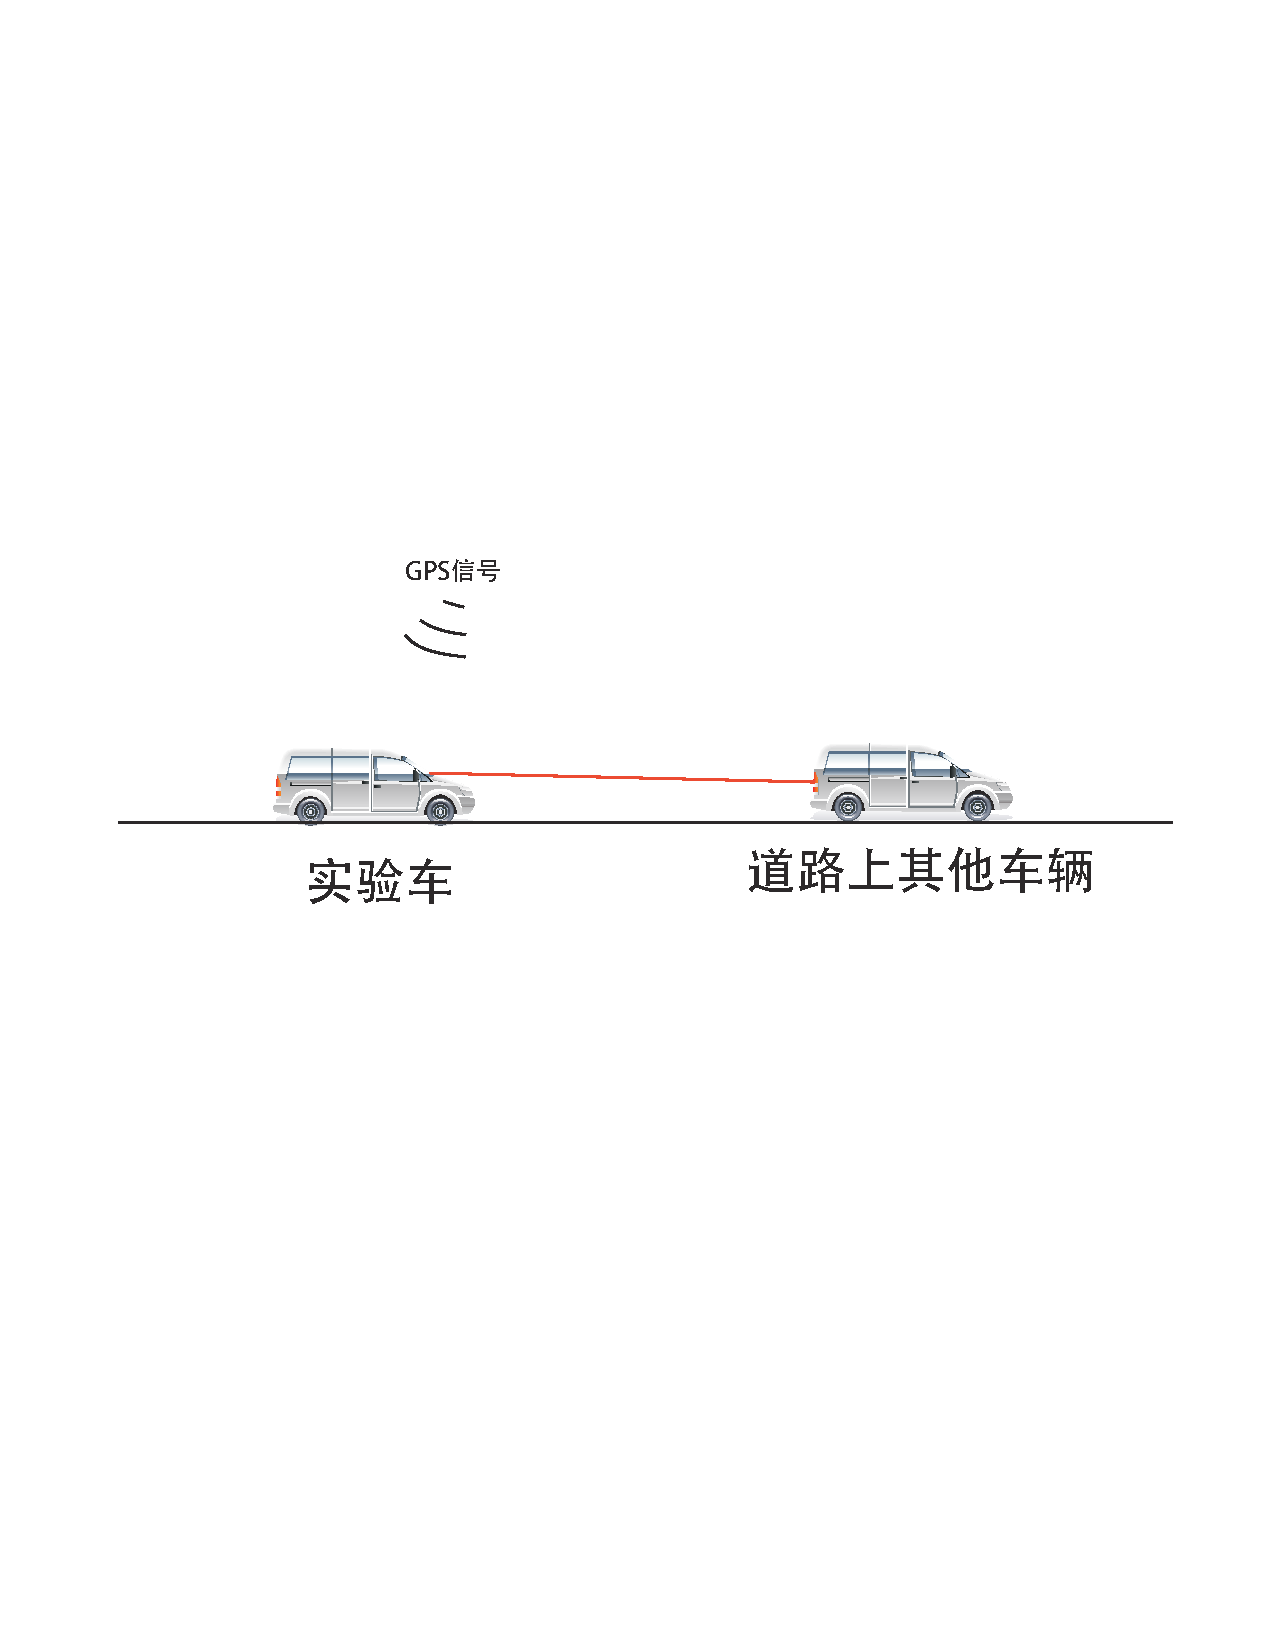
\includegraphics[width=0.7\linewidth]{test_illus}
	\caption{实验系统示意图(红色线条代表激光)}
	\label{test_illus}
\end{figure}


\subsection{数据采集软件}

数据采集软件主要起到变量实时运算和时间同步处理的功能。

通过实验仪器直接获取的数据只有实验车辆实时经纬度与前车和后车的实时距离,要得到所需要的实验车辆速度、前车相对速度、前车速度、后车相对速度、后车速度等数据,可以通过以下运算得到。
GPS定位仪输出的是WGS-1984经纬度坐标,在此坐标下计算行驶距离的公式为:
\begin{equation}
D = 2R{\rm{asin}}(\sqrt {\sin _{}^2(\frac{{{l_1} - {l_2}}}{2}) + \cos ({l_1})\cos ({l_2}){{\sin }^2}(\frac{{{w_1} - {w_2}}}{2})} )
\end{equation}
其中 $D$(m)为经纬度坐标点( ${l_1},{w_1}$)和(${l_2},{w_2}$)之间的距离, $R$为地球半径,取6378137m。设定GPS每秒钟返回一个数据,当前车辆的瞬时速度 (单位m/s)计算公式为:$v = D'$
设$\Delta t$为记录前后两个坐标点的时间差,本车加速度 $a$($m/s^2$)则通过本车速度计算得到,计算公式为:
\begin{equation}
a = \frac{{{v_1} - {v_2}}}{{\Delta t'}}
\end{equation}
其中$v_1$,$v_2$分别为相邻的两瞬时速度(单位m/s), $\Delta {t'}$为两个瞬时速度的时间差(单位s)。激光测距仪直接输出的是本车车头与前车车尾之间的间距,前车与本车的相对速度 (m/s)计算公式如下:
\begin{equation}
{v_r} = \frac{{{d_2} - {d_1}}}{{\Delta {t^{''}}}}
\end{equation}
其中$d_1$,$d_2$为相邻两个车间距(单位m), $\Delta t''$为两个相邻车间距对应的时间差(单位s),又${v_r} = {v_f} - {v_b}$,其中${v_f}$为前车速度(单位s), ${v_b}$为后车速度(单位s),故前车的速度为:
\begin{equation}
{v_f} = {v_r} + {v_b}
\end{equation}

运算得到所关心变量以后,时间同步处理通过GPS的校时功能,将GPS轨迹点和其他变量对应地标上时间点并输出保存。

\section{实验与数据采集}
\subsection{实验对象}
实验对象分为专业驾驶人与非专业驾驶人。其中,专业驾驶人主要选取长期从事驾驶工作,或驾龄7年且累计行程10万公里以上的驾驶人;非专业驾驶人主要选取非特定职业,驾龄不足7年或累计行程不足10万公里的驾驶人。选取的专业驾驶人与非专业驾驶人都尽可能来自各行各业,覆盖各年龄层,最终的样本包括10名专业驾驶人和16名非专业驾驶人。
\subsection{实验路线}
实验路线的选取考虑了以下条件。首先,道路条件方面包含单向两车道城市道路与单向三车道城市道路,且路段上开口较少,有机非分隔带,机动车行驶受非机动车和行人干扰较小,路面情况良好;其次,交通条件方面有足够大的交通流量,但是不至于造成长时间的拥堵,道路上行驶的车型以小汽车为主。

经过实地调查,本实验选取的实验路段为:南京市龙蟠中路-瑞金路-御道街-中山东路一线。其中龙蟠中路为双向六车道;瑞金路东西向为三车道,西东向为两车道;御道街靠近瑞金路一段为双向四车道,靠近中山东路一段为双向六车道;中山东路为双向四车道。该路段全天交通流量均较大且高平峰时流量相差不大,平峰时段车流量满足要求,高峰时段不造成长时间拥堵,车辆跟驰特征明显,比较符合实验要求。具体线路如\autoref{route}所示。

\begin{figure}[htpb]
	\centering
	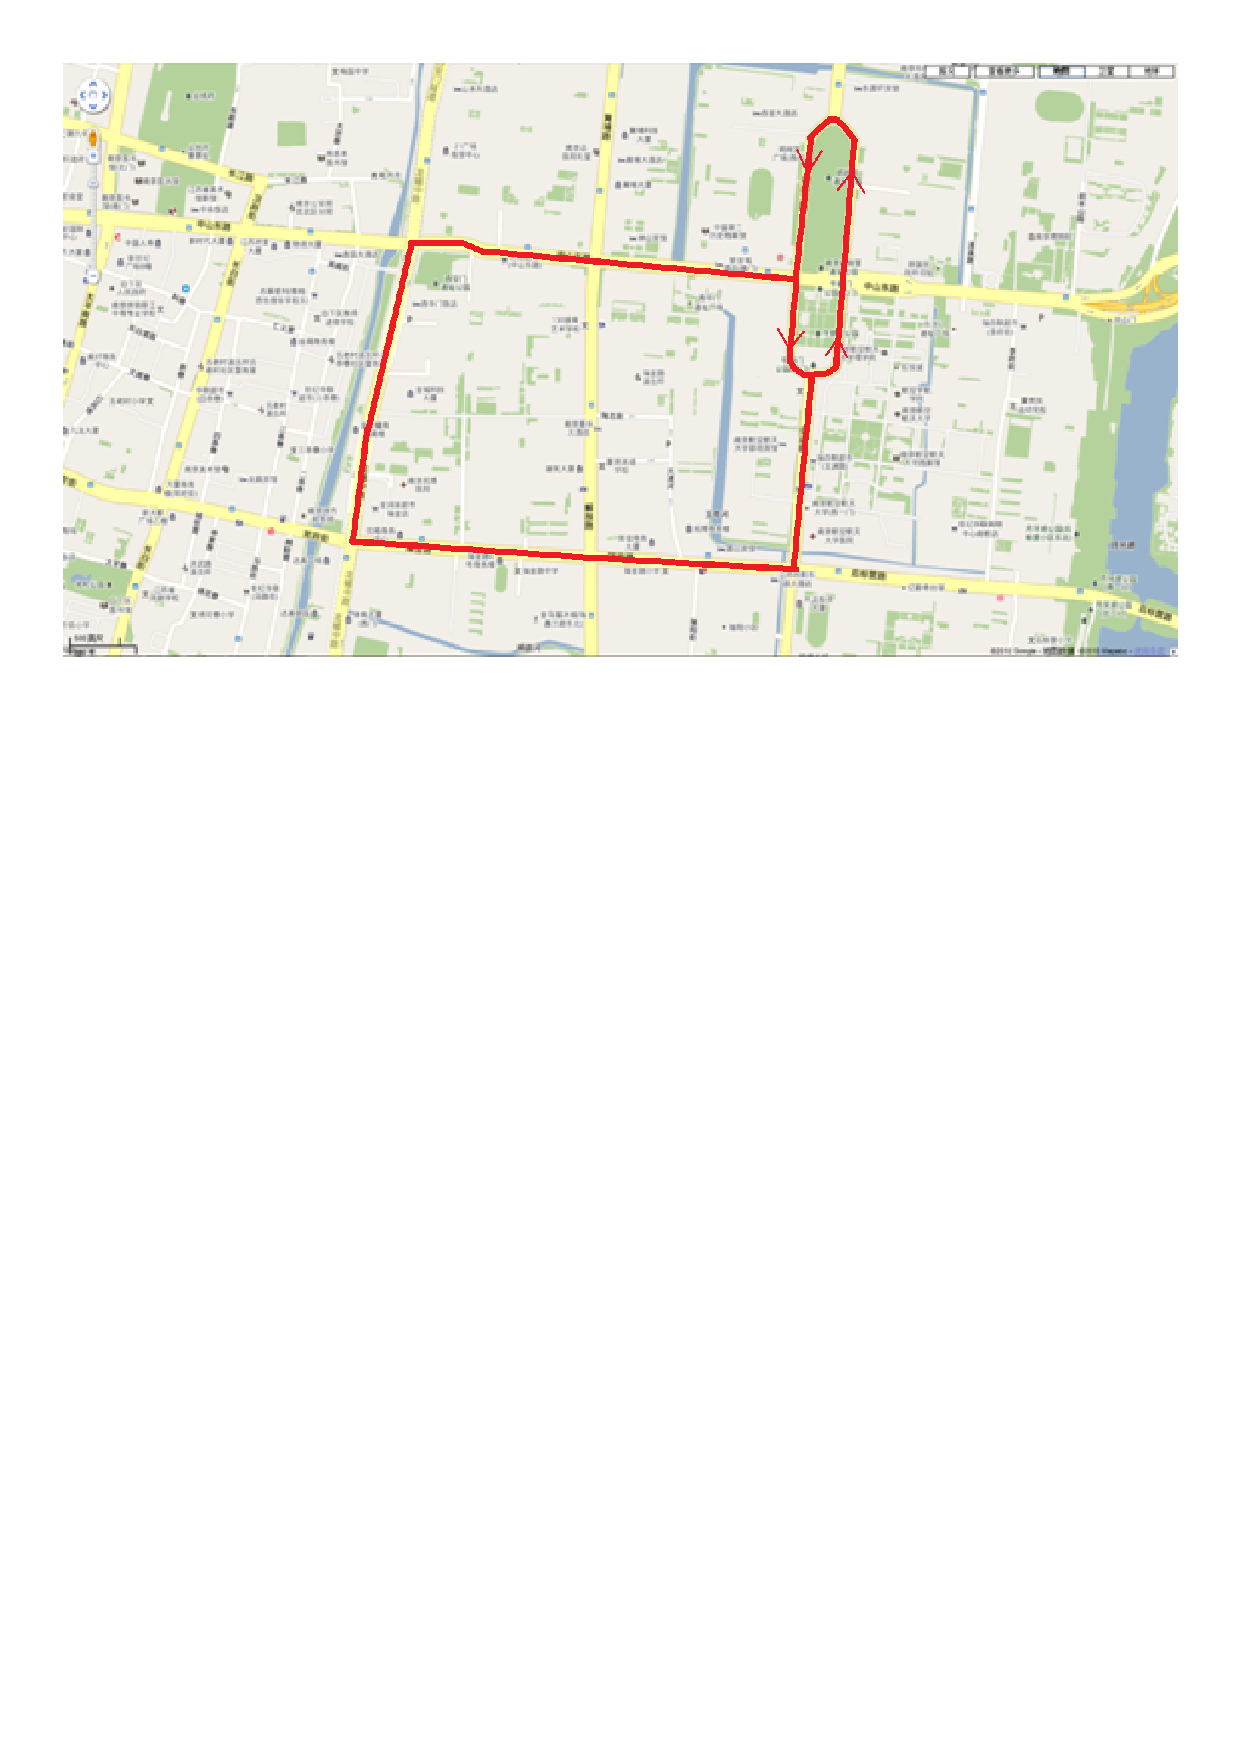
\includegraphics[width=0.7\linewidth]{route}
	\caption{实验路线示意图}
	\label{route}
\end{figure}

\subsection{实验条件}
实验选择在天气良好、光线充足的条件下进行。所选取的时间段主要在车流量较大但不造成长时间拥堵的时候,能够满足车辆跟驰的要求。经过调查发现,实验路段上,工作日与非工作日的交通流量变化不大,交通流量与高平峰时间段相对固定。最后根据所选取路段的交通流量以及高平峰的时间,本论文实验时间定为8:00——11:00和13:00——18:00。
\subsection{实验过程}
实验过程中,在按照既定路线驾驶行车前,向每个实验参与者说明实验的目的、设备及用途、既定的路线等,并指示其放松并安装日常习惯驾驶。实验于2010年9月进行,历时共15天。
%其次,将我们准备好的《驾驶人特性实验调查问卷》与《驾驶人安全意识调查表》给实验参与者填涂。
%具体表格(暂略待补)
%然后,开始进行路上实验,由一名实验参与者按照事先拟定的路线,驾驶实验车辆,沿着龙蟠中路——瑞金路——御道街——中山东路——龙蟠中路一圈后调头,再沿着龙蟠中路——中山东路——御道街——瑞金路——龙蟠中路行驶。
%最后,保存数据,结束一次实验。
%准备下一个实验参与者进行实验。



\section{本章小结}
本章介绍了本文数据来源所使用的实验方法,包括硬件组成,设备原理和数据采集软件。并描述了实验过程。
















%\begin{table}[htbp]
% \centering
% \caption{Add caption}
% \begin{tabular}{cccc}
%   \addlinespace
%    \toprule
%    Face database & Yale  & Caltech & ORL \\
%    \midrule
%    Number of training & \multicolumn{ 1}{c}{5} & \multicolumn{ 1}{c}{3} & \multicolumn{ 1}{c}{3} \\
%    samples per class  & \multicolumn{ 1}{c}{} & \multicolumn{ 1}{c}{} & \multicolumn{ 1}{c}{} \\
%    \bottomrule
%    \end{tabular}
%  \label{tab:addlabel}
%\end{table}
